\documentclass[10pt,a4paper]{paper}
\usepackage[latin1]{inputenc}
\usepackage{amsmath}
\usepackage{amsfonts}
\usepackage{amssymb}
\usepackage{graphicx}
\usepackage{fancyvrb}
\usepackage[a4paper, total={7in, 8in}]{geometry}
\title{Guide into the WIOD R-package}
\author{Sybren Deuzeman}

\begin{document}
	\maketitle
	
	\section{Introduction}
	
	\section{Installing the WIOD R-package}
	
	\section{Load International Input Output Tables}
	
	The WIOD R-package comes with an easy way to easily import international input-output tables into our R environment. The data can be loaded in such a way that the different versions of international input-output tables can be used right away without the need to get the data into a workable format yourself. The data is, however, not delivered with the package as this would mean that the package becomes very large. Instead, the data is stored separately on the internet and can be downloaded with some pre-build functions. 
	
	There are two ways to use the WIOD R-package. The first is to download the data from the internet at use and the other is to create and use a local copy. Creating a local copy is advisable, since the data-files are relatively large. Since loading from the internet is the easiest to explain, we start with that. After that, we explain how to make a local copy and use that in a way very similar to loading from the internet.
	
	\subsection{Load from the Internet}
	
	In this section, we explain how to load the data using the internet and how the data itself is formatted. We start by downloading a international input-output table for a single year and version. Using this, we will explain the contents of an international. Next, we will explain how to load in a whole database of international input-output tables that is better suited for time-series analysis.
	
	\subsubsection{Load a Single IOT}
	\label{subsec:loadsingleiot}
	To load a single IOT, we can use the following function call \texttt{iot <- load\_iot("<version>", year)}.  For example, we can load international input-output table for 2000 from the World Input Output Database (WIOD) 2016 edition international input-output table using
	\begin{Verbatim}
	iot <- load_iot("WIOD2016", 2000)
	\end{Verbatim}
	
	This will load a large list that called \texttt{iot}. This list is the basic building block of the package as the build-up of these lists are the same for all different versions.
	
	The content of this list is:
	\begin{itemize}
		\item \texttt{I}: a matrix with the intermediate inputs use in one industry from another industry.
		\item \texttt{FD}: a matrix with different the final demand uses of the products of a sector. 
		\item \texttt{S}: a vector with the gross output of the sectors.
		\item \texttt{VA}: the value added of the sectors.
	\end{itemize}	
	
	After that follow some parameter that can be used by the program.
	\begin{itemize}
		\item \texttt{c}: number of countries in the input-output table
		\item \texttt{cf}: number of countries to which final demand goes.
		\item \texttt{n}: the number of industries. 
		\item \texttt{f}: the number of final demand categories. 
		\item \texttt{year}: the year for which the international input-output table is.
		\item \texttt{version}: the version of the international input-output table.
		\item \texttt{countries}: vector with the countries in the order in which they appear in the input-output table.
		\item \texttt{industries}: vector with the industries in the order in which they appear in the input-output table.
	\end{itemize}
	
	\begin{figure}[t]
	\centering
	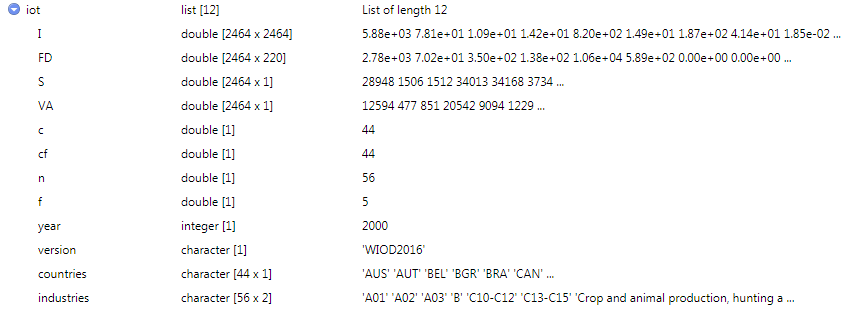
\includegraphics[width=\linewidth]{content_iot}
	\caption{The content of a Input-Output Table after loading it}
	\label{fig:contentiot}
	\end{figure}

	
	\subsubsection{List of IOTs}
	To obtain time-series, it is useful to load lists of IOTs instead of working with different single IOTs. The package comes with a function that can load such a list. To use the functions to export the results, one should also such lists instead of separate IOTs.
	
	One can load such a list of IOTs via the following command \texttt{iots <- load\_iots("<version>")}. To load the whole WIOD 2016 database at once, one can use the following code:
	\begin{Verbatim}
	WIOD2016 <- load_iots("WIOD2016").
	\end{Verbatim}
	Sometimes you would only want to load the data for a few years. We can do so by adding a vector with the years you want. To download the data of the WIOD 2016 database from 2005 to 2010 only, the following can be used:
	\begin{Verbatim}
	WIOD2016_0510 <- load_iots("WIOD2016", 2005:2010)
	\end{Verbatim}
	
	\subsection{Load Extra Data}
	In some cases, supplemental data needs to be downloaded. For example, the WIOD project database also consists of the Socio-Economic Accounts. This data can be added to the list via one of two functions \texttt{load\_extra\_iot} or \texttt{load\_extra\_iots}. To load the Socio-Economic Accounts (SEA) to the already loaded \texttt{iot}, you can use:
	\begin{Verbatim}
	iot <- load_extra_iot(iot, "SEA")
	\end{Verbatim} 
	To load the Socio-Economic Accounts to a list of IOTs, i.e. to the already loaded \texttt{WIOD2016}, you can use:
	\begin{Verbatim}
	WIOD2016 <- load_extra_iots(WIOD2016, "SEA")
	\end{Verbatim}
	
	\subsection{Make a Local Copy}
	To use a local copy instead of data from the internet, one can first download the data from the internet. To do so, first set the directory where to store the international input-output tables using the \texttt{change\_dir\_data} function. For example, if one wants to store the data \texttt{c:\\data\_wiod}, use
	\begin{Verbatim}
	change_dir_data("c:/data_wiod")
	\end{Verbatim}
	Then, to download a full dataset and its social-economic accounts, for example the WIOD 2016 data, one can use:
	\begin{Verbatim}
	download_iots("WIOD2016")
	download_extra_iots("SEA", "WIOD2016")
	\end{Verbatim}
	After this, the downloaded data can be accessed in the same way as using the online data. To access the data again in a new session, use \texttt{change\_dir\_data} again. Even manually downloading is not necessary. After using \texttt{change\_dir\_data} is used, the load functions described in the sections above will, if possible, automatically download missing data. Hence,
	\begin{Verbatim}
	change_dir_data("c:/data_wiod")
	WIOD2016 <- load_iots("WIOD2016")
	\end{Verbatim}
	is enough to download and load all the data from the World Input-Output Database 2016.
	
	If you do no longer want to use local data, you can simply change back to using internet data via:
	\begin{Verbatim}
	reset_dir_data()
	\end{Verbatim}
	
	\section{Use International Input Output Tables}
	We want to use International Input-Output Tables to generate new measures. For this, one can either build an own function as described in \ref{sec:ownfunction} or use one of the build-in functions. The functions are build to work with a single international input-output table. However, with the function \texttt{on\_iots} one can also use these functions on list of international input-output tables.
	
	\subsection{Use of package with single IOT}
	Here, we describe how to use a function and how these functions will behave in general. To do so, we consider the build-in function gii. This function  calculates the global import intensity of a specific sector as in [[CITATION]]. We will use function with \texttt{iot}, which we already downloaded:
	\begin{Verbatim}
	iot <- gii(iot)
	\end{Verbatim}
	We store the output of this function to the same list that we also used as argument for the function. We could have stored it as well into another list, which will then be a copy of the old list with new results added.
	
	\begin{figure}
	\centering
	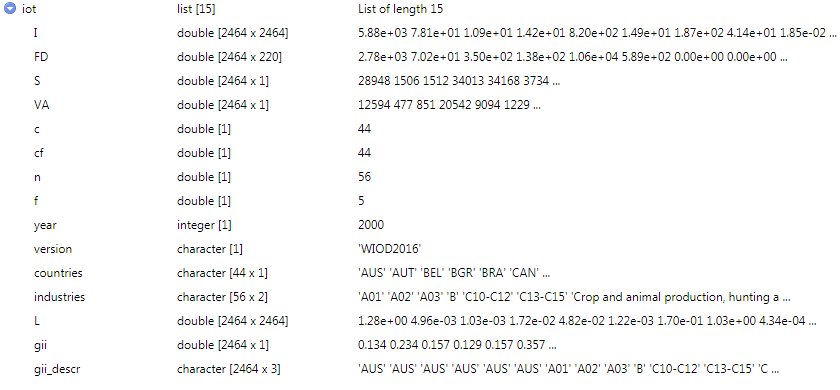
\includegraphics[width=1\linewidth]{content_iot_function}
	\caption{Content of \texttt{iot} after the command}
	\label{fig:contentiotfunction}
	\end{figure}

	In figure \ref{fig:contentiotfunction}, we show the contents of \texttt{iot} after using the function \texttt{gii}. Most part is as discussed in section \ref{subsec:loadsingleiot}. Three elements are added. The first is \texttt{L}, which is the Leontief inverse. As calculating the Leontief inverse is computationally intensive, we store the Leontief inverse for later use. Second, the element \texttt{gii} is added. In \texttt{gii}, the results of our calculations are stored. Third \texttt{gii\_descr} is added. In \texttt{gii\_descr}, we store the description of the data that can be used by our export functions.
	
	The function \texttt{gii} also has two other arguments, namely \texttt{regions} and \texttt{industries}. These arguments add region and industry categories to \texttt{gii\_descr}. To get a region categorization, one can use the function \texttt{countrycat}. As an example, we add a NAFTA and BeNeLux categorization:
	\begin{Verbatim}
	NAFTA <- c("USA", "MEX", "CAN")
	BENELUX <- c("BEL", "NLD", "LUX") 
	regions <- countrycat(list(NAFTA, BENELUX), iots)
	\end{Verbatim} 
	to create a region categorization. Finally, we use the \texttt{regions} argument as
	\begin{Verbatim}
	iot <- gii(iot, regions = regions)
	\end{Verbatim}
	to include the region categories to the data description.
	
	\subsection{Use of package with list of IOTs}
	If we use a list of international input-output tables, we can use the function \texttt{on\_iots}. The function \texttt{on\_iots} executes a function on all the input-output tables in the list. To use the function \texttt{gii} on all elements of the list \texttt{WIOD2016}, we can use
	\begin{Verbatim}
	WIOD2016 <- on_iots(gii, WIOD2016)
	\end{Verbatim}
	To add extra arguments, like te region categories as before, one can add extra arguments to the end of the function call, i.e.:
	\begin{Verbatim}
	WIOD2016 <- on_iots(gii, WIOD2016, regions = regions)
	\end{Verbatim}
	
	\section{Export Results}
	In the package, results are stored in a list of lists. Without some help, it is therefore not easy to extract the data for further analysis. To help us, the package includes two functions: \texttt{export\_dataframe} and \texttt{export\_csv}. The first function exports the data to an R dataframe. The second function exports the data into a CSV file, such that the results can be loaded into another program for further analysis.
	\subsection{Export to Dataframe}
	
	To extract the earlier calculated global import intensities from \texttt{WIOD2016} into a dataframe, we can use:
	\begin{Verbatim}
	gii_df <- export_dataframe("gii", WIOD2016)
	\end{Verbatim}
	This will generates a dataframe in ``wide'' format. Every year will have a separate column with its data. We can also export the data into ``long'' format. This does not store every year into a different variable, but gives the year for which it is in a separate column. This can be done via:
	\begin{Verbatim}
	gii_df_long <- export_dataframe("gii", WIOD2016, long = TRUE)
	\end{Verbatim}
	This function can be used to export the results of different functions. To add, for example, the total final demand for certain sectors, one can use
	\begin{Verbatim}
	WIOD2016 <- on_iots(fd_total, WIOD2016)
	gii_fvas_df <- export_dataframe(c("gii", "fd_total"), WIOD2016)
	\end{Verbatim}
		
	If \texttt{gii} and \texttt{fd\_total} would not have been of the same length, an error occurs. Further, the data description for \texttt{gii} will be used as this was the measure that is at the first position.
	
	\subsection{Export into a CSV file}
	The function \texttt{export\_csv} shares the same basic setup. The most simple way to use it is
	\begin{Verbatim}
	export_csv("gii", WIOD2016)
	\end{Verbatim}
	If one runs this code, a window will open to ask where to store the results. One can also add the file-path or filename directly via the directory argument:
	\begin{Verbatim}
	export_csv("gii", WIOD2016, directory = "C://Some/Dir/and/File.csv")
	\end{Verbatim}
	\section{Make Your Own Functions}
	\label{sec:ownfunction}
	The strength of this package is that you only need to write the function, while the rest of the package takes care of managing the data. The functions can be written for a single input-output table, while the rest of the package makes it easy to obtain results for a whole database of input-output tables.
	
	To aid in writing your own functions, we show the source code of the \texttt{gii} function:
	\begin{Verbatim}
	gii <- function(iot, regions = "None", industries = "None"){
		# Do necessary preliminary calculations
		A <- coefficient(iot)
		iot <- leontief(iot)
	
		# Get results
		temp = matrix(1, iot$c, iot$c) # Create a c x c matrix with ones
		for (i in 1:iot$c){
			temp[i,i]=0 # make the diagonal into 0's
		}
		S = kronecker(temp, matrix(1, iot$n, iot$n)) 
		result <- t(colSums(S * A) %*% iot$L) 
		
		# Store results to the list
		iot$gii <- result	
		iot$gii_descr <- countryindustry_descr(iot, regions, industries)
		
		# Return the list
		return(iot)
	}	
	\end{Verbatim}
	The code is split in four parts. We will discuss these parts shortly.
	
	\paragraph{Do necessary preliminary calculations} Here some necessary calculations are done. We need to find the so called coefficient matrix and the Leontief matrix to calculate the GII. We do not store the coefficient matrix, \texttt{A} in the IOT list, but we do so for the Leontief inverse \texttt{L}. We want to calculate the Leontief inverse only once as it is computationally heavy and therefore we store it for later use. Finding the coefficient matrix is not computationally heavy, so we can find it every time we need it.
	
	\paragraph{Get results} Here, we do some calculations to get the necessary results. One can use elements from the IOT list using \texttt{iot\$element}. Observe that we use \texttt{colSums()} to find the sum over all elements of the columns. In R, element-wise manipulation is generally much faster than matrix manipulations. One should thus avoid matrix manipulation. 
	
	\paragraph{Store results to the list}
	The results are stored to the list of the input-output table via  \texttt{iot\$gii <- result}. Next, we add a description via another function \texttt{iot\$gii\_descr <- countryindustry\_descr(iot, regions, industries)}. 
	
	\paragraph{Return the list} The list \texttt{iot} that contains now, next to the original content, the Leontief inverse, the GII calculations and its accompanying data description is returned as the result of the function call.
	\end{document}